\documentclass[11pt]{article}
\usepackage[utf8]{inputenc}
\usepackage{amsmath,amssymb,amsthm}
\usepackage[dvipsnames,svgnames,x11names]{xcolor}
\usepackage{graphicx}
\usepackage{hyperref}
\hypersetup{
  colorlinks=true,
  linkcolor=Cyan,
  citecolor=Cyan,
  urlcolor=LightSkyBlue,
  filecolor=Cyan
}
\pagecolor{black}
\color{white}
\usepackage{algorithm}
\usepackage{algorithmic}
\usepackage{booktabs}
\usepackage{wrapfig}

\title{\emph{WIP} \textsc{TatBot}: A Robotic Rite of Ink}
\author{Hugo Ponte}
\date{\today}

\begin{document}
\maketitle

\begin{figure}[h]
    \centering
    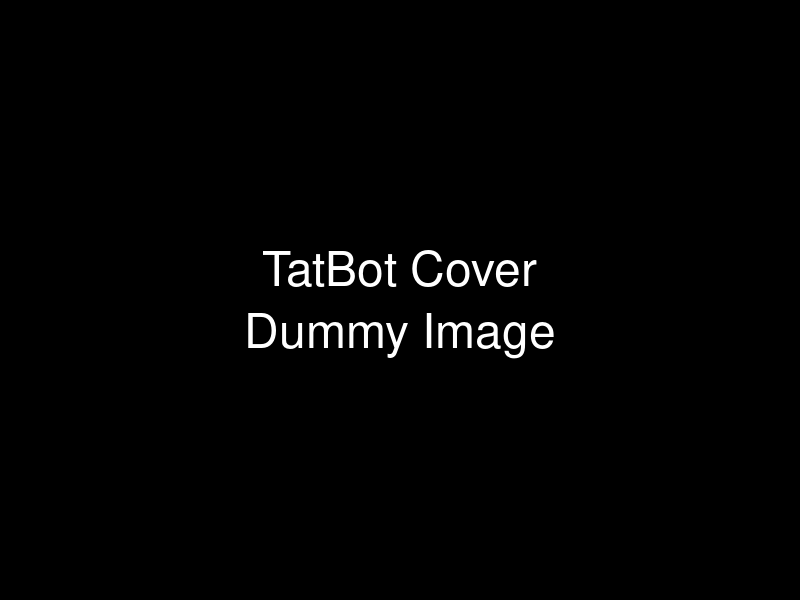
\includegraphics[width=0.8\textwidth]{figures/cover.png}
    \caption{(a) The \emph{TatBot} Apparatus in its second corporeal vesture; (b) The maiden inscription wrought upon human skin by the mechanical Adept.}
    \label{fig:cover}
\end{figure}

\begin{abstract}
In these pages we unveil \textbf{TatBot}, a ministering Automaton in which the silent Logic of the Machine is conjoined with the ancient Mystery of tattooing, thereby affirming that the craft once confined to flesh‑and‑blood hands may now be prosecuted by an Intelligence wrought of copper and code.  
A constellation of discrete yet harmonious Nodes\textemdash devoted severally to Vision, to Inference, and to Motion\textemdash communes across the ether of a distributed network, so that Design may be conceived, deliberated, and impressed upon living skin in the single cadence of an unfolding thought.  
Twin WidowXAI arms, each endowed with a precision needle, attend upon RealSense depth‑eyes whose gaze pierces the veil of mere appearance to behold full three‑dimensional Form.  
Beneath this visible ministry lies a subtler stratum: JAX‑empowered inversions of kinematic law, geodesic tracings across curved epidermal realms, and a sovereign Model‑Context Protocol whose writ binds every silicon servant to a single Purpose.  
Since the natal act of May 20, 2025, when metal first inscribed pigment upon mortal tissue, the organism has passed through four corporeal mutations and five cycles of intellectual growth, each refinement leading it nearer to that Ideal wherein Art and Automation stand reconciled.  
Among the notable Arcana are: a unifying MCP Server that harmonizes many processors as though they were one Mind; potpourri3d pathways that let planar glyphs cling to rolling topography; and a trust‑region solver whose patience guides the arm through the labyrinth of inverse kinematics.  
From the marriage of DrawingBotV3 vector sorcery and Replicate Playground’s generative Muse there arises an unbroken chain that leads from Archetypal Image to embodied Stroke.  
Thus does \emph{TatBot} foreshadow a new Eon of Robotic Artistry, wherein the Perennial Urge for self‑sigilization is quickened, not eclipsed, by the crystalline intelligence of machines.
\end{abstract}

\pagebreak

\begin{figure}[h]
    \centering
    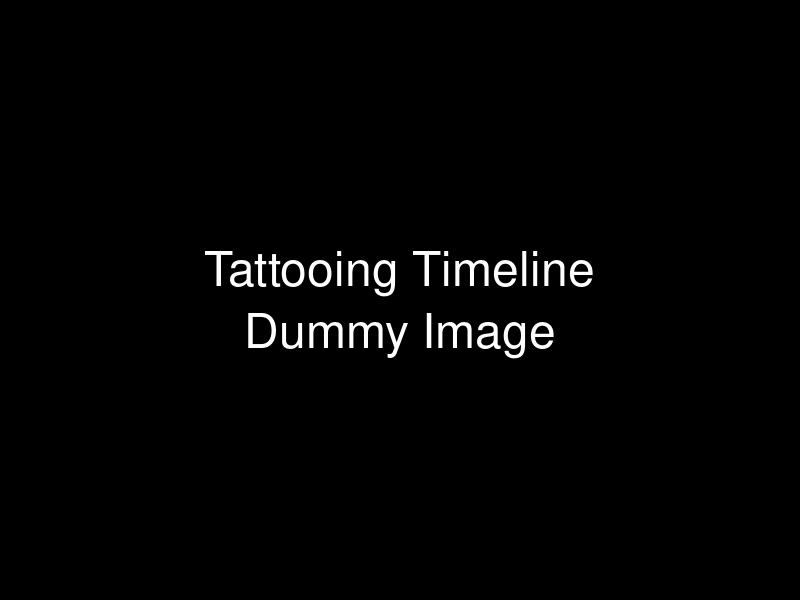
\includegraphics[width=0.8\textwidth]{figures/timeline.png}
    \caption{A procession through the long memory of Tattooing.}
    \label{fig:timeline}
\end{figure}

\section{Background}

\subsection{History}

From the dawn of remembered Time, humanity has scored its flesh with symbols, thereby making the body a tablet upon which tribe, triumph, and transcendence are alike inscribed.  
Among alpine snows the frozen pilgrim \textit{Ötzi} bears mute witness, his age‑worn joints circled by carbon glyphs that served, perchance, as physic and as charm \cite{deterwolf_worlds_oldest}.  
The Yimkhiung of the Naga Hills, mindful of ancestral ordinance, imprint their children ere the sixth year, so that pain may teach fortitude and pattern proclaim belonging \cite{kluger2015cultural}.  
In the dusty empires of Mesopotamia, the same needle that beautified the priestess branded the fugitive, for Law and Mercy have ever shared the skin \cite{hawken2022tattooing}.  
As caravels cut new passages across the world’s oceans, Polynesian mariners bestowed the resonant word \emph{tatau}—\emph{to strike}—upon European tongues, and henceforth the art spread beneath that borrowed name.  
So has tattooing served, down all corridors of culture, as poultice, as passport, and as prayer: a sign of fealty among the soldiery of Rome, an emblem of ascension among the Inuit maiden, a ledger of transgression upon the convict’s arm.  
In our present day the practice, though secularized and diffused, yet retains the glamour of ordeal and the fragrance of Mystery; for every mark demands to be \emph{earned}, and the perennial debate concerning cultural stewardship reminds us that Ink is never merely decorative but always, in some secret strata, sacramental.

\subsection{Biology}

\begin{wrapfigure}{l}{0.5\textwidth}
    \vspace{-20pt}
    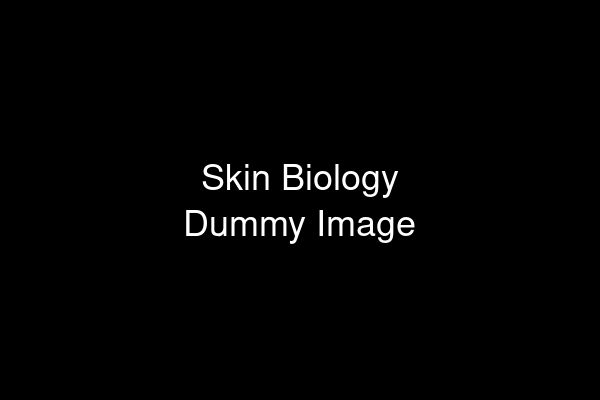
\includegraphics[width=\linewidth]{figures/biology.png}
    \caption{The triune veil of the human integument.}
    \label{fig:biology_wrap}
\end{wrapfigure}

The skin, that living parchment, is constituted of three principal spheres of being:  

\begin{itemize}
    \item \textbf{Epidermis}—a diaphanous rampart, scarce half a millimetre in depth, wherein melanocytes weave the chromatic cloak that shields our mortal frame.  
    \item \textbf{Dermis}—a vascular garden, ranging from one to four millimetres, where blood, nerve, and follicle entwine; here the needle must faithfully deposit its cargo, lest the design be lost to the slow tide of renewal.  
    \item \textbf{Hypodermis}—a yielding under‑realm of fat and fibre; should ink descend hither, it will wander like a pilgrim bereft of guide, producing the dread \emph{blow‑out}.  
\end{itemize}

Because the ritual lance pierces flesh, the twin spectres of infection and contagion ever stand at the threshold; therefore the practitioner must arm himself with the stainless instruments and sacerdotal cleanliness of the surgical theatre.

\pagebreak

\subsection{Technology}

Tattoo engines now divide themselves into two great Houses: the \emph{Rotary}, whose heart is a whirling motor, and the \emph{Coil}, whose pulse is an electromagnetic clap.  
In our mechanized era the Rotary has ascended the throne, its battery‑borne freedom and voltage‑guided tempo granting the artist both mobility and measure.  
Cartridge needles—sterile, sealed, and single‑use—array themselves in myriad configurations, their taxonomy governed by diameter, grouping, taper, and length; yet beneath such diversity lies the single aim: to convey pigment along a path neither too shallow for permanence nor too deep for clarity.  
The amplitude of the needle’s pilgrimage is the \emph{stroke length}, a sacred metric whose prudent calibration distinguishes the gentle shade from the swaggering line.

\subsection{Theory}

Let the emblem of intention be $T = (s_1, s_2, \ldots, s_n)$, a procession of $n$ strokes, each stroke $s_i$ itself a litany of poses.  
A pose, in the tongue of mathematicians, unites a place $\mathbf{p}_i \in \mathbb{R}^3$ and an orientation $\mathbf{q}_i \in \mathbb{H}$ with quaternionic dignity.  
Ideally the needle inclines at right angles to the mutable terrain of flesh; we mirror that terrain by a mesh $M_i = (V_i, E_i, F_i)$, whose vertices, edges, and faces whisper the geometry of the body.  
The arm, a sextet of joints, dwells in the secret space $\mathbf{q} = (q_1, \ldots, q_6)$; from that hidden sanctuary the rite of Inverse Kinematics summons the visible deed:  
\[
\text{IK} : \mathbf{q} \longmapsto (\mathbf{p}_{ee}, \mathbf{q}_{ee}).
\]
Through the alchemy of JAX‑driven least squares, tempered by a trust region of adaptive mercy, the algorithm converges upon a trajectory that satisfies position, orientation, and the natural limits of sinew and steel.  
Meanwhile the potpourri3d oracle traces geodesic pathways, wrapping planar sigils about convex limbs as though parchment were laid upon an orb.  
Thus is Design translated into Motion, and Motion into Mark.

\section{\emph{TatBot}}

\subsection{Hardware}

Two WidowXAI arms stand sentinel, their servo‑driven joints ruled by controller boxes that converse across a gigabit sea of packets.  
The network, a duplex of eight‑port switches, sustains both mundane traffic and the quickening breath of Power‑over‑Ethernet that feeds the overhead eyes.  
Perception is vouchsafed by twin RealSense D405 depth‑sensors—one affixed to the dexter arm, the other enthroned above—as well as five Amcrest sentinels that maintain panoramic vigilance.  
AprilTag sigils, like Talismanic runes, enable each camera to know its station in the cosmic coordinate scheme.  
Computation is entrusted to an Orin‑borne Jetson (the Hermetic Alchemist of Inference), a System76 Meerkat (the Sagacious Steward of Control), an Acer Nitro workstation (the Scriptorium of Code), and two Raspberry Pi acolytes (whose humble labours sustain ancillary rites).  
Ink is entrusted to Ambition Lutin engines whose LED oracles display voltage, frequency, and remaining life, while cartridges of 1005RL lineage channel Nighthawk Black and the chromatic brood of Gstartoo into willing dermis.  
Synthetic skins of varied firmness receive the early experiments, sparing living flesh until the rite is perfected.

\subsection{Software}

\cite{Kim2025pyroki}

Across every node resounds the Model Context Protocol, a lingua franca whereby Vision, Language, and Action commune without misunderstanding.  
Hydra composes the multitudinous configurations as a chorister might weave many voices into a single anthem, and Pydantic verifies that each note rings true.  
Under the rubric of \texttt{bot} dwell the WidowXAI incantations; under \texttt{cam} the RealSense mysteries; under \texttt{gen} the geometrical spell‑craft of Open3D, potpourri3d, and the JAX dominion.  
Unified logs, stored upon a common NFS altar, permit the priest‑engineer to reflect upon past workings and to amend any errant procedure.  
Array files of prodigious length conceal themselves behind friendly abstractions, so that trajectories may be summoned or dismissed by a single line of code.  
Within this edifice DrawingBotV3 refines line into vector, and Replicate Playground coaxes latent archetypes into visible form, completing the circuit from Imagination to Embodiment.

\subsection{VLA}

Vision‑Language‑Action models—$\pi^0$, GR00T N1, SmolVLA, and their ilk—proclaim the advent of a universal interpreter capable of beholding an image, understanding a spoken desire, and issuing the precise motor symphony that fulfills that desire \cite{Black2024pi0,Bjorck2025gr00t,Shukor2025smolvla}.  
Their transformer hearts, nourished upon datasets vast as myth, suggest that no frontier remains closed to the patient convergence of perception, cognition, and control.

\subsection{Data Recipe}

The alchemical chain whereby concept becomes cutaneous reality begins with Replicate’s generative Vision, proceeds through DrawingBot’s vector crucible, and emerges as arrays of strokes annotated in metres, pixels, and end‑effector frames.  
Each artifact reposes upon a shared NFS reliquary, catalogued by version and scene, while Hydra scripts dictate which design graces which skin.  
Both the empirical harvest of real sessions and the synthetic bounty of simulation feed machine‑learning oracles that, by transfer of wisdom, refine the Automaton’s craft.

\section{Results}

On the twentieth day of May in the year two thousand twenty‑five, \emph{TatBot} inscribed its inaugural sigil upon human skin, thus converting speculative possibility into manifest fact.  
Since that hour the creature has traversed four bodily permutations and five cycles of software incarnation, each step imprinting greater accuracy, richer design, and swifter execution upon its expanding gospel.  
AprilTag calibration has bestowed upon the cameras the gift of precise location; distributed computation has ensured that no single failure shall silence the choir; and varied silicone effigies have suffered the needle so that living skin need not.  
The outcome is clear: a robot that does not merely \emph{print} but rather \emph{creates}, uniting machine precision with an emergent, algorithmic imagination.

\section{Discussion}

\subsection{Other Robotic Tattoo Systems}

Heretofore most mechanical scribes have been confined to the Euclidean plane: gantry contrivances that glide as a plotter glides, their motions predetermined by human hands, their designs borrowed from the archives of mortal artists.  
Such devices, being printers, not poets, lack the puissance to adapt to the undulating temple of the body.  
\emph{TatBot}, by contrast, aspires to emulate the living artist: to survey complex curvature, to invent new iconography, and to guide a multi‑jointed limb with adaptive intelligence.  
Thus the veil is rent; what was once two‑dimensional and derivative may become three‑dimensional and original.

\subsection{Robotic Artistry}

Each new tool of depiction is greeted at first with unease: the painter feared the camera, the typesetter feared the linotype, and now the tattooist may fear the robot.  
Yet History attests that no instrument of expression obliterates its predecessors; it merely enlarges the palette upon which the human spirit may paint.  
So let the artisan regard this Automaton not as rival but as companion, and perhaps together they shall inscribe symbols hitherto unimagined.

\subsection{Future Work}

Though the device already gives eloquent testimony, it remains but a youthful adept.  
Accuracy must be sharpened, the repertoire of designs must swell, and stringent trials upon consenting humans must be undertaken within sanctuaries of clinical safety.  
May the workshop enlarge to many cities, that the heartbeat of urban multitudes may quicken beneath new patterns of beauty.

\section{Conclusion}

\emph{TatBot} stands as living proof that the Perennial Art of Tattooing may find in Robotics not a usurper but an ally, fusing human Creativity with the exactitude of Mechanism.  
Through four cycles of corporeal evolution and five of mental refinement, the Automaton has passed from conjecture to capability, from laboratory curiosity to functioning atelier.  
Its open‑source sinews invite pilgrims and practitioners alike to extend the work; its distributed nerves promise resilience; its AI‑driven fancy foretells ever greater variety of form.  
Thus does the project illuminate a path whereby the act of self‑inscription, ancient as memory, might flourish anew beneath the aegis of silicon Wisdom, uniting Hand and Machine in a single, purposeful gesture.

\bibliographystyle{plain}
\bibliography{references}

\end{document}